% \chapter{Axion--Like Particles search with ultracold neutrons}
%
% \label{ch:axions}

\chapter{Introduction}
\label{ch:axions-intro}





% \section{Motivation}
% \begin{figure}
%   \centering
%   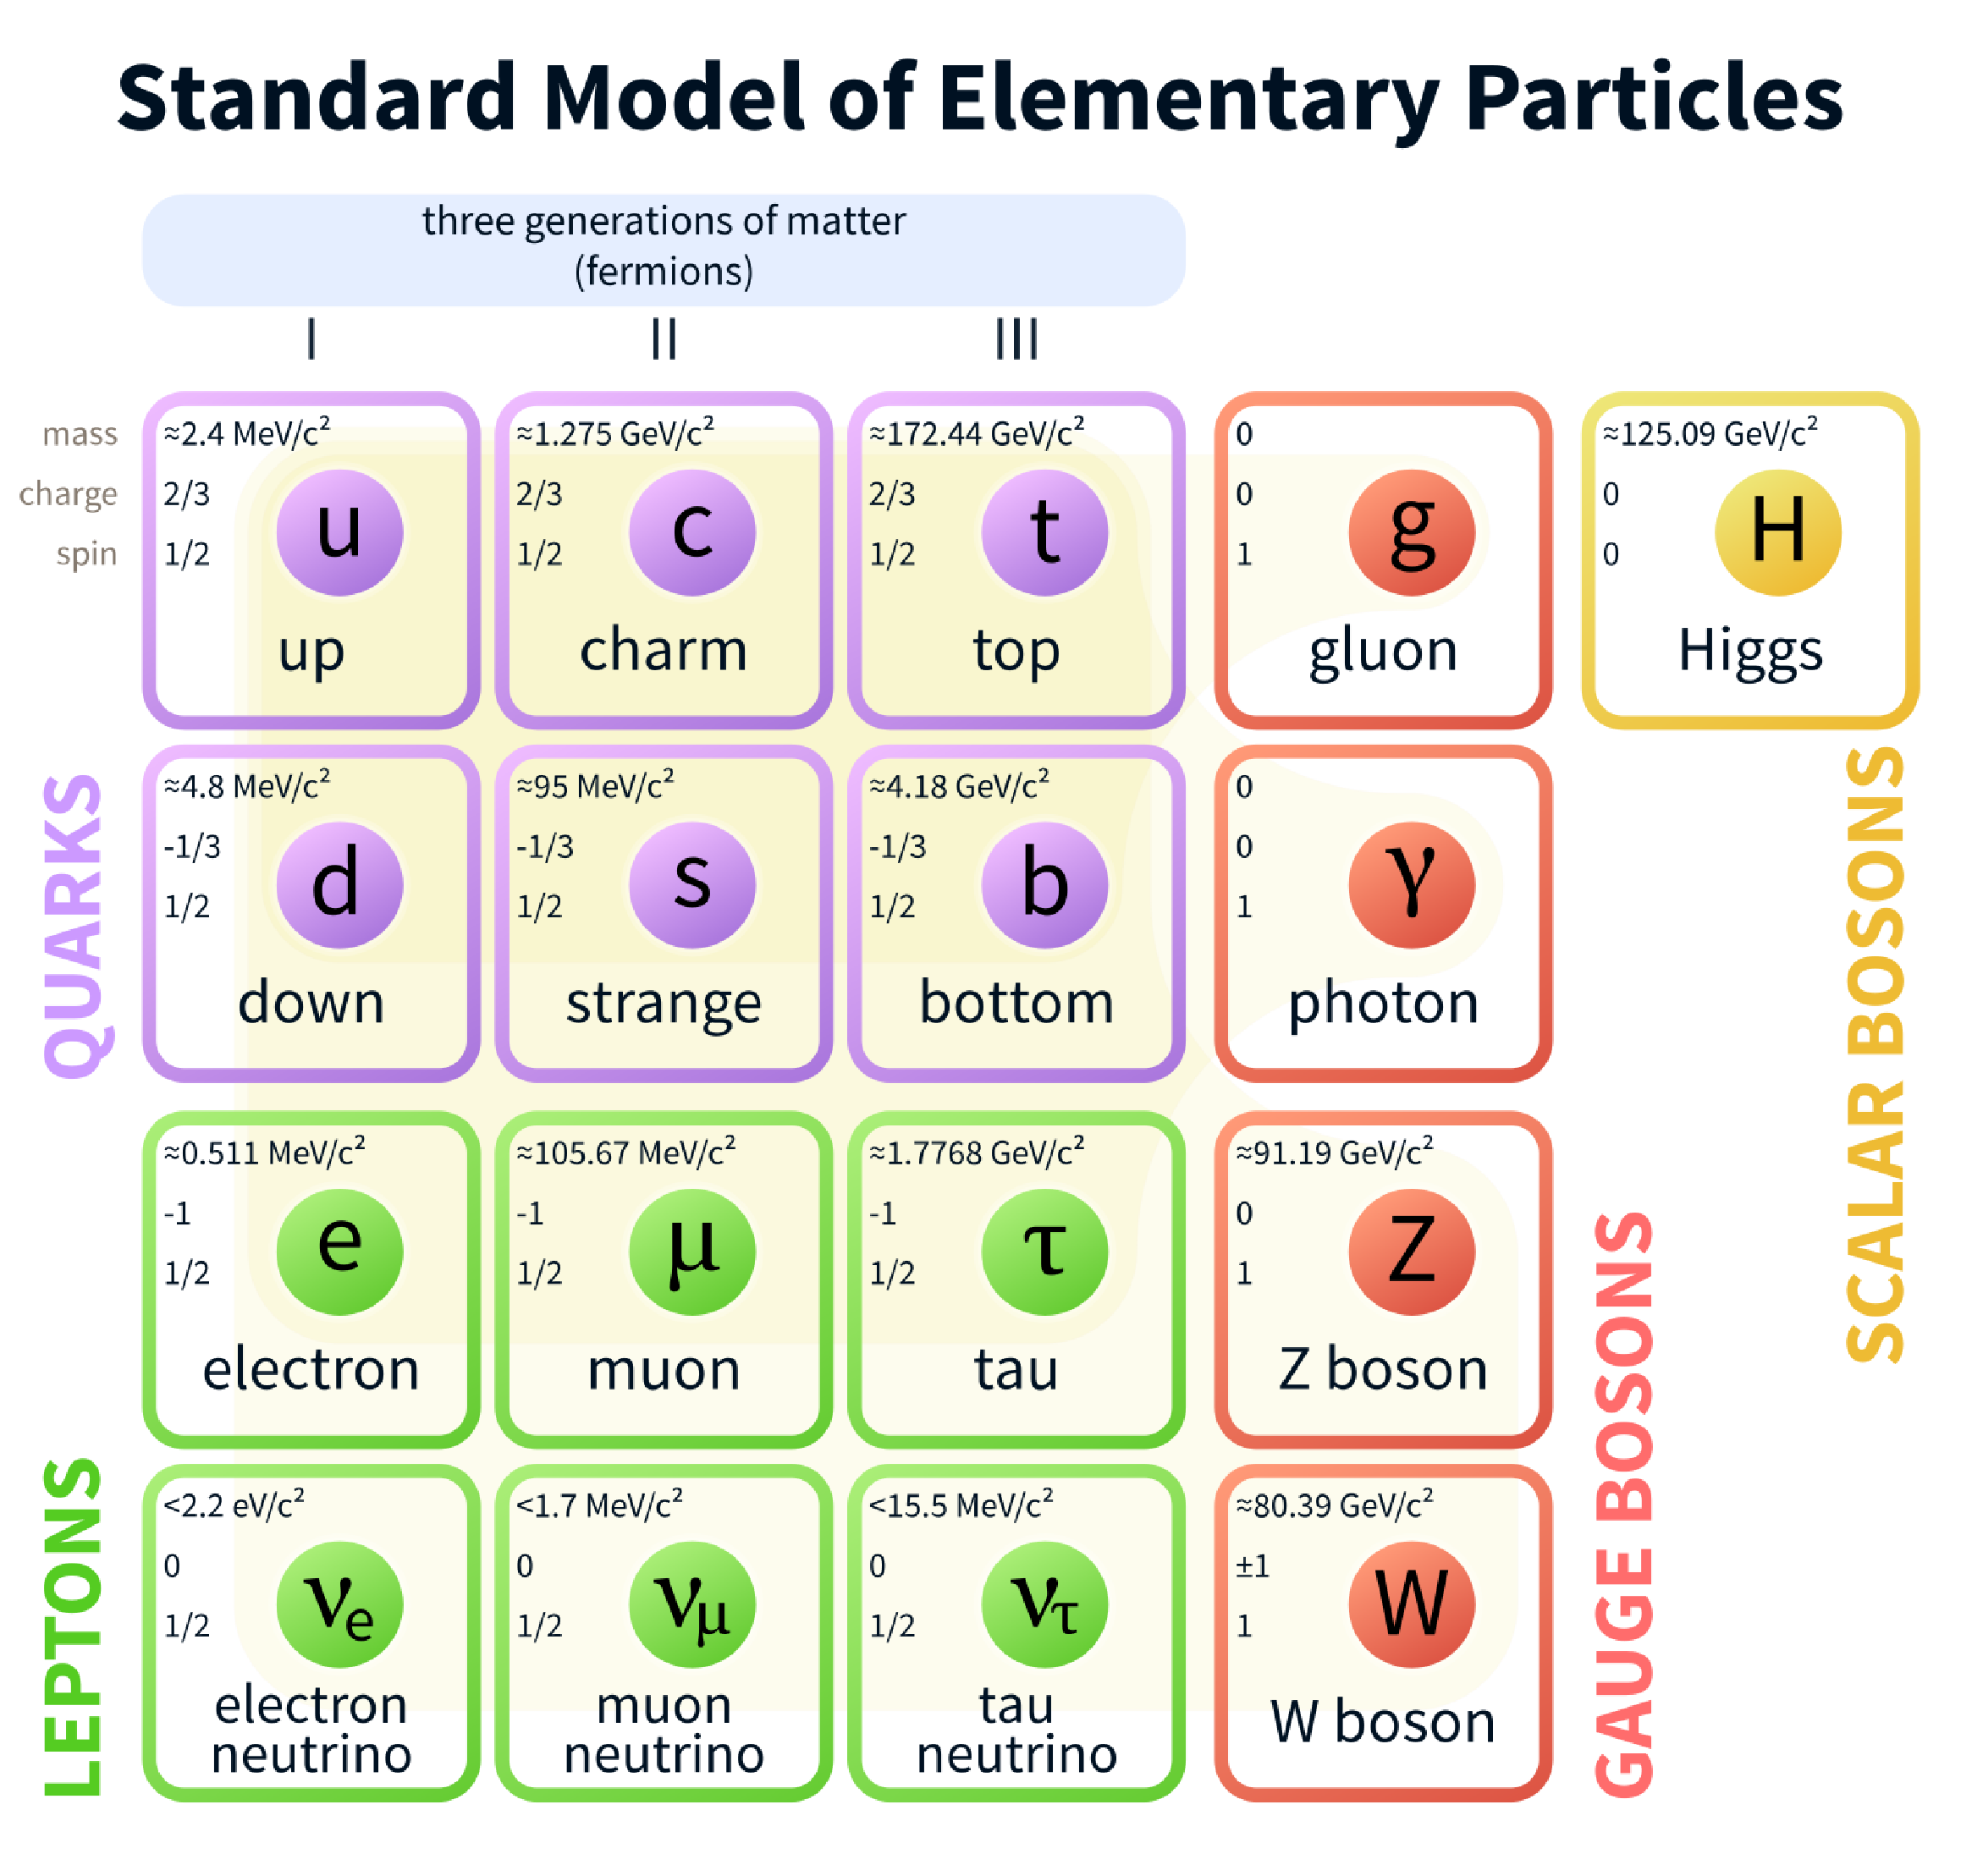
\includegraphics[width=0.5\linewidth]{gfx/axions/Standard_Model_of_Elementary_Particles.pdf}
%   \caption{Standard Model particles - known matter.}
%   \label{fig:axions_SM_particles}
% \end{figure}
% The twentieth century is a success story of the Standard Model of Particle Physics, whtested in laboratories with extraordinary precision \note{cite something cool}.

% ost of them falling into two categories: Weakly Interacting Massive Particles (WIMPs) and axions. Axions, in contrast to WIMPs, would be very light, but abundant. And could be 

% As early as 1884 Lord Kelvin has estimated the number of bodies in our Milky Way galaxy based on the velocity distribution and noted that most of them we do not see. \note{cite}

% Over the next hundred years this approach, pioneered by Zwicky (ref) has been extended. Measuring the \emph{rotation curves} of the galaxies, the relation between the velocity of the stars in their motion around the galactic centre and the distance from it, provided a way to estimate the distribution of the mass. Gravitational lensing is another method.

% It is the fundamental curiosity that drives the desire to understand what is Dark Matter made of.

% Axions and WIMP are searched for with fundamentally different techniques. WIMP detectors, like XENON (ref) try to detect a single interaction signature of a WIMP particle with the mass of the detector. The detectors are massive, many tons, and almost background-free. In attempts to detect axions one looks for very weak signals coming from the omnipresent bulk axion matter.

% We will focus on axions.


% This part is concerned with a search for a signature of an axion dark matter in the data measured by the nEDM experiment at PSI\@. The signature would be an oscillation in the array of the measured ratios of the precession frequencies of the neutrons and ${}^{199}$Hg atoms, as measured during normal nEDM data taking.

% The method of choice to quantify oscillations in the unevenly sampled array is the least-squares periodogram~\cite{Scargle1982}. In the next chapters we introduce the periodogram, discuss its properties and develop statistical methods for an oscillation search.

% % Then, the analysis itself is presented. 

% % methodology is developed, then the data.

% Here say, that we first develop the methods on a simple example in the next chapter. A search for an oscillating nEDM~\ref{eq:nEDM_axion} is presented.

% Then the next chapter is\ldots


\section{Theoretical background}
\marginpar{This section is largely based on Ref.\,\cite{PhysRevX.7.041034}.}
Based on astrophysical and cosmological observations an estimated 26\% of the total energy density of the Universe and 84\% of its mass content is dark matter (DM)~\cite{Planck2015}. The observations give hints about the amount and distribution of DM, for example via rotational curves or gravitational lensing~\cite{ApJ1990}, but the micro-scale properties of DM, in particular its constituents, remain unknown.

Among the candidates for DM is an axion, a new scalar particle, initially proposed to solve the strong QCD problem (the strong sector in the Standard Model appears to be fine-tuned to be $CP$-even)~\cite{PhysRevLett.38.1440,PQ1977B,Weinberg1978,Wilczek1978,Kim1979,Zakharov1980,Zhitnitsky1980B,Srednicki1981}. Later, it has been since generalised to axion-like particles, or simply axions~\cite{Witten1984,Conlon2006,Witten2006,Arvanitaki2010,Arias2012,Marsh2015Review}. Light ($m_a \lesssim \SI[per-mode=symbol]{0.1}{\electronvolt\per\clight\squared}$) axions can be produced efficiently via non-thermal production mechanisms, such as vacuum misalignment in the early Universe~\cite{Preskill1983cosmo,Sikivie1983cosmo,Dine1983cosmo}. They fill the universe as almost stationary particles and through gravity participate in the galaxy formation. As they fall, they gain speed ($\approx \SI[per-mode=symbol]{300}{\kilo\metre\per\second}$) and, as bosons, condensate into a coherent oscillating field ($\Delta\omega / \omega \sim \num{e-6}$)~\cite{Marsh2015Review}
\begin{equation}
  a = a_0 \, \cos\left(\frac{ m_a c^2 }{\hbar} \ t\right) \ .
\end{equation}
The frequency of the oscillation is set by the mass of the axion.

Due to its effects on structure formation~\cite{Khlopov1985}, ultra-low-mass axion DM in the mass range $\SI{e-24}{\electronvolt} \lesssim m_a \lesssim \SI{e-20}{\electronvolt}$ has been proposed as a DM candidate that is observationally distinct from, and possibly favourable to, archetypal cold DM~\cite{Hu2000,Marsh2014,Schive2014,Marsh2015Review,Hui2017}.
The requirement that the axion de Broglie wavelength does not exceed the DM size of the smallest dwarf galaxies and consistency with observed structure formation~\cite{Marsh2015B,Schive2015,Marsh2017} give the lower axion mass bound $m_a \gtrsim \SI{e-22}{\electronvolt}$, if axions comprise all of the DM\@. However, axions with smaller masses can constitute a sub-dominant fraction of DM~\cite{Hlozek15}.

It is reasonable to expect that axions interact non-gravitationally with standard-model particles.
Direct searches for axions have thus far focused mainly on their coupling to the photon (see the review~\cite{Axion-Review2015} and references therein).
% **WHY WAS THIS HERE?  (MALCOLM)** coherently oscillating spin-dependent effects due to the
%\note{BL: We should cite: The here described experiment obtained a new limit on axion-like particles using ultracold neutrons \cite{Afach2015Exotic}.}
%\note{YS: In the earlier (long) version of this paper, we actually had a reference to this paper and several other papers on related applications of ultracold neutrons to look for new physics. In the process of shortening the paper, the paragraph containing these references was cut out, but perhaps we could restore the references somewhere in the paper.}
Recently, however, it has been proposed to search for the interactions of the coherently oscillating axion DM field with gluons and fermions, which can induce oscillating electric dipole moments (EDMs) of nucleons~\cite{Graham2011} and atoms~\cite{Stadnik2014A,Roberts2014A,Roberts2014B}, and anomalous spin-precession effects~\cite{Flambaum2013Patras,Stadnik2014A,Graham2013}.
The frequency of these oscillating effects is dictated by the axion mass, and more importantly, these effects scale linearly in a small interaction constant~\cite{Graham2011,Stadnik2014A,Roberts2014A,Roberts2014B,Flambaum2013Patras,Graham2013}, whereas in previous axion searches, the sought effects scaled quadratically or quartically in the interaction constant~\cite{Axion-Review2015}.

In the present work, the focus is on the axion-gluon and axion-nucleon couplings:
\begin{align}
\label{Axion_couplings}
\mathcal{L}_{\textrm{int}} = \frac{C_G}{f_a} \frac{g^2}{32\pi^2} a G^{b}_{\mu \nu} \tilde{G}^{b \mu \nu}  - \frac{C_N}{2f_a} \partial_\mu a ~ \bar{N} \gamma^\mu \gamma^5 N \, ,
\end{align}
where $G$ and $\tilde{G}$ are the gluonic field tensor and its dual, $b=1,2,\ldots,8$ is the  color index, $g^2 / 4 \pi$ is the color coupling constant, {\color{black}$N$ and $\bar{N} = N^\dagger \gamma^0$ are the nucleon field and its Dirac adjoint,} $f_a$ is the axion decay constant, and $C_G$ and {\color{black}$C_N$} are model-dependent dimensionless parameters.
Astrophysical constraints on the axion-gluon coupling in (\ref{Axion_couplings}) come from Big Bang nucleosynthesis~\cite{Blum2014,StadnikThesis,Stadnik2015D}:~$m_a^{1/4} f_a / C_G \gtrsim 10^{10}~\textrm{GeV}^{5/4}$ for $m_a \ll 10^{-16}~\textrm{eV}$ and $m_a f_a / C_G \gtrsim 10^{-9}~\textrm{GeV}^{2}$ for $m_a \gg 10^{-16}~\textrm{eV}$, assuming that axions saturate the present-day DM energy density,
and from supernova energy-loss bounds~\cite{Graham2013,Raffelt1990Review}:~$f_a / C_G \gtrsim 10^6 ~\textrm{GeV}$ for $m_a \lesssim 3 \times 10^{7}~\textrm{eV}$.
{\color{black}Astrophysical constraints on the axion-nucleon coupling in (\ref{Axion_couplings}) come from supernova energy-loss bounds~\cite{Raffelt1990Review,Raffelt2008LNP}:~$f_a / C_N \gtrsim 10^9 ~\textrm{GeV}$ for $m_a \lesssim 3 \times 10^{7}~\textrm{eV}$, while existing laboratory constraints come from magnetometry searches for new spin-dependent forces mediated by axion exchange~\cite{Romalis2009_NF}:~$f_a / C_N \gtrsim 1 \times 10^4 ~\textrm{GeV}$ for $m_a \lesssim 10^{-7}~\textrm{eV}$. }

The axion-gluon coupling in (\ref{Axion_couplings}) induces the following oscillating EDM of the neutron via a chirally-enhanced 1-loop process~%\footnote{Interaction (\ref{Axion_couplings}) also non-perturbatively induces a mass $m_a \approx 6C_G\,\mu\text{eV} \cdot (10^{12}\text{ GeV}/f_a)$.
%Axions with masses much smaller than this are theoretically fine-tuned.}
\cite{tuningfootnote,Witten1979,Witten1979B,Pospelov1999}:
%\note{KK: merge to [42-44]}
\begin{equation}
\label{eq:nEDM_axion}
d_\mathrm{n}(t) \approx +2.4 \times 10^{-16} ~ \frac{C_G a_0}{f_a} \cos(m_a t) ~ e \cdot \textrm{cm} \, .
\end{equation}
The axion-gluon coupling in (\ref{Axion_couplings}) also induces oscillating EDMs of atoms via the 1-loop-level oscillating nucleon EDMs and tree-level oscillating P,~T-violating intra-nuclear forces (which give the dominant contribution)~\cite{Stadnik2014A,Flambaum1984EDM,Flambaum1984EDMB}.
In the case of $^{199}$Hg, the oscillating atomic EDM is~\cite{Stadnik2014A,StadnikThesis,Flambaum1985EDM,Flambaum1985EDMB,Flambaum2002EDM,Dmitriev2003A,Dmitriev2003B,Dmitriev2005,Engel2005,Engel2010}:
\begin{equation}
\label{199Hg-EDM_axion}
d_{\textrm{Hg}}(t) \approx +1.3 \times 10^{-19} ~ \frac{C_G a_0}{f_a} \cos(m_a t) ~ e \cdot \textrm{cm} \, ,
\end{equation}
which is suppressed compared to the value for a free neutron (\ref{eq:nEDM_axion}), as a consequence of the Schiff screening theorem for neutral atoms~\cite{Schiff1963}.
%\note{KK: a question to our theory friends: Eqns. (2) and (3) suggest that $d_n$ and $d_\textrm{Hg}$ would have the same sign. Is this intended or are we rather talking about the modulus?}
%\note{YS: Yes, the same signs for $d_n$ and $d_\textrm{Hg}$ are intended here.}
%\note{MR: Should we explicitly point that out then?}
%\note{YS: I think this would be a good idea. We could explicitly add "+" signs in both Eqs. (2) and (3) to remove any ambiguity.}
%\note{CG: Might be good to comment that the Hg contribution is quite safely assumed to be negligible compared to the neutron for the purposes of this paper.}
The amplitude of the axion DM field, $a_0$, is fixed by the relation $\rho_a \approx m_a^2 a_0^2 /2$.
In the present work, we assume that axions saturate the local cold DM energy density $\rho_{\mathrm{DM}}^{\mathrm{local}} \approx 0.4~\textrm{GeV/cm}^3$~\cite{Catena2010}.




%Crucially, the constant amplitude of the axion DM field, $a_0$, is fixed by the known DM density at the location of the Earth, $\rho_{\mathrm{DM}}=\approx 0.4~\textrm{GeV/cm}^3$ \cite{Catena2010} (when reporting constraints on the couplings we assume axions make up all the local DM).


% Our experiment is also sensitive to the time-dependent energy shifts induced by the derivative coupling of an oscillating galactic axion DM field, $a = a_0 \cos(m_a t - \vtr{p}_a \cdot \vtr{r})$, with spin-polarised nucleons in (\ref{Axion_couplings}):
The derivative coupling of an oscillating galactic axion DM field, $a = a_0 \cos(m_a t - \vtr{p}_a \cdot \vtr{r})$, with spin-polarized nucleons in (\ref{Axion_couplings}) induces time-dependent energy shifts according to:
\begin{equation}
\label{potential_axion-wind}
H_{\textrm{int}} (t) = \frac{C_N a_0}{2 f_a} \sin(m_a t) ~ \vtr{\sigma}_N \cdot \vtr{p}_a \, .
\end{equation}
The term $\vtr{\sigma}_N \cdot \vtr{p}_a$ is conveniently expressed by transforming to a non-rotating celestial coordinate system (see, e.g.,~\cite{Kostelecky1999}):
\begin{align}
\label{sigma-p_a_2}
\vtr{\sigma}_N \cdot \vtr{p}_a  &= \hat{m}_F f(\sigma_N) m_a |\vtr{v}_a|  \notag \\
& \times \left[\cos(\chi) \sin(\delta) + \sin(\chi) \cos(\delta) \cos(\Omega_{\textrm{sid}} t - \eta) \right] \, ,
\end{align}
where $\chi$ is the angle between Earth's axis of rotation and the spin quantization axis ($\chi = 42.5 ^\circ$ at the location of the PSI), $\delta \approx -48 ^\circ$ and $\eta \approx 138 ^\circ$ are the declination and right ascension of the galactic axion DM flux relative to the Solar System~\cite{NASA2014web}, $\Omega_{\textrm{sid}} \approx 7.29 \times 10^{-5}~\textrm{s}^{-1}$ is the daily sidereal angular frequency, $\hat{m}_F = m_F / F$ is the normalized projection of the total angular momentum onto the quantization axis, and $f(\sigma_N) = +1$ for the free neutron, while $f(\sigma_N) = -1/3$ for the $^{199}$Hg atom in the Schmidt (single-particle) model.


% A transition paragraph about why we need a method to look in the frequency space and need to calculate the periodograms.


\section{Overview}
This part is concerned with a search for a signature of an axion dark matter in the data measured by the nEDM experiment at PSI\@. The signature would be an oscillation in the array of the measured ratios of the precession frequencies of the neutrons and ${}^{199}$Hg atoms, as measured during normal nEDM data taking.

The method of choice to quantify oscillations in the unevenly sampled array is the least-squares periodogram~\cite{Scargle1982}. In the next chapters we introduce the periodogram, discuss its properties and develop statistical methods for an oscillation search.

% Then, the analysis itself is presented. 

% methodology is developed, then the data.

Here say, that we first develop the methods on a simple example in the next chapter. A search for an oscillating nEDM~\ref{eq:nEDM_axion} is presented.

Then the next chapter is\ldots